\section{Auswertung}
\label{sec:Auswertung}

\subsection{Phasenempfindlicher Gleichrichter}
\label{sec:Gleichrichter}

Einem eingetselltes sinusförmiges Signal von $U_{sig} = 300 mV$ mit einer Frequenz von $1 kHz$,
wird mit einem Referenzsignal $U_{ref} = 1.65 V$ identischer Frequenz gemischt. 
Am Preamplifier ist ein Gain von 10 eingestellt, welcher die Amplitude um das Zehnfache erhöht.
Beim Bandpass wurde für das beste Ergebnis die Einstellung Bess. gewählt, sowie m Low-Pass 0.3 gewählt.
Die richtigen Einstellungen erhielt man durch ausprobieren aller und Vergleich der Ergebnisse.
Durch Phasenverschiebung der beiden Signale werden Folgende Ausgangssignale erzeugt.

\begin{figure}
  \centering
  \begin{subfigure}{0.3\textwidth}
    \centering
    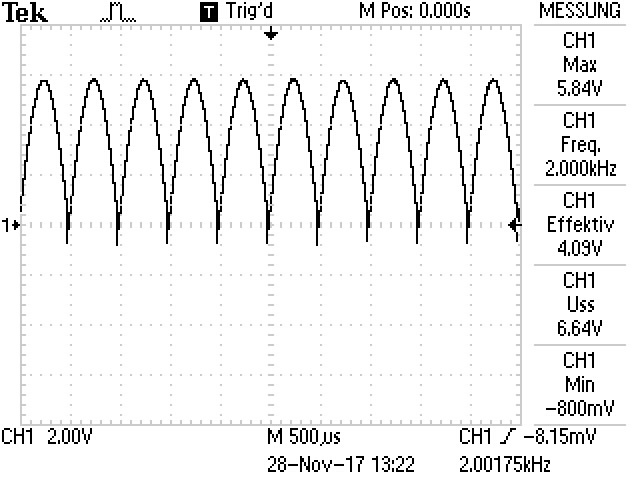
\includegraphics[height=3cm]{data/Phase1.jpg}
    \caption{0 Grad.}
    \label{fig:Phase1}
  \end{subfigure}
  \begin{subfigure}{0.3\textwidth}
    \centering
    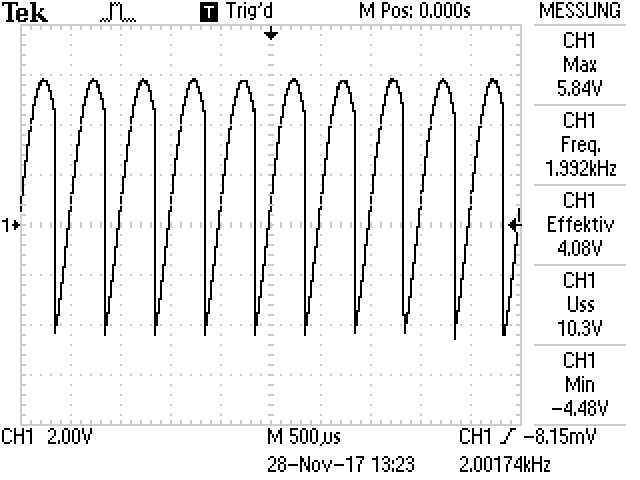
\includegraphics[height=3cm]{data/Phase2.jpg}
    \caption{45 Grad.}
    \label{fig:Phase2}
  \end{subfigure}
  \begin{subfigure}{0.3\textwidth}
    \centering
    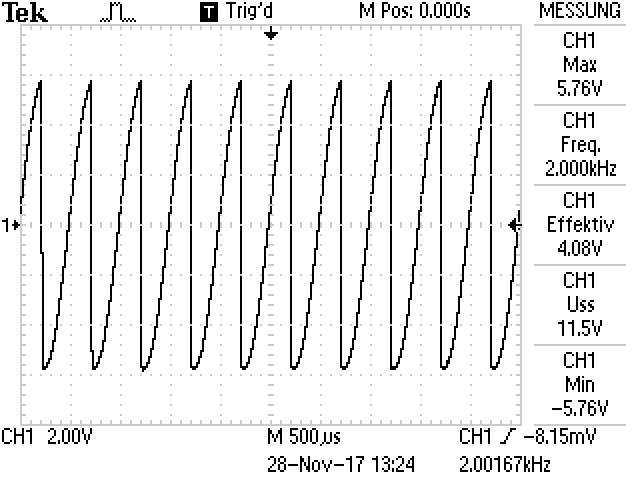
\includegraphics[height=3cm]{data/Phase3.jpg}
    \caption{90 Grad.}
    \label{fig:Phase3}
  \end{subfigure}
  \begin{subfigure}{0.3\textwidth}
    \centering
    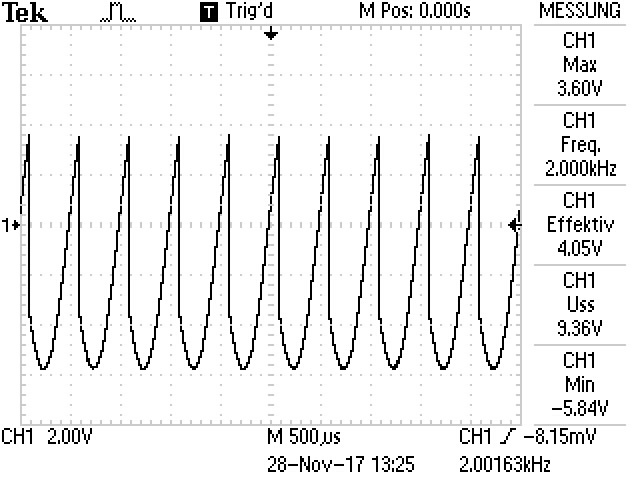
\includegraphics[height=3cm]{data/Phase4.jpg}
    \caption{135 Grad.}
    \label{fig:Phase4}
  \end{subfigure}
  \begin{subfigure}{0.3\textwidth}
    \centering
    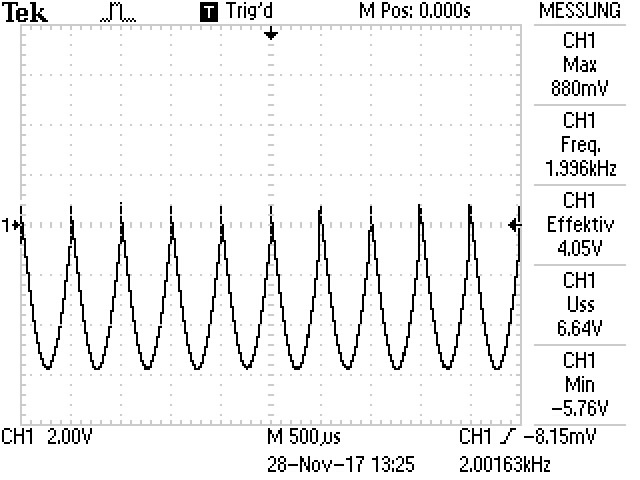
\includegraphics[height=3cm]{data/Phase5.jpg}
    \caption{180 Grad.}
    \label{fig:Phase5}
  \end{subfigure}
  \caption{Phasenverschiebungen}
  \label{fig:Phasen}
\end{figure}

Es wird eine Umkippung der Amplitude nach 180 Grad festgestellt. 
Mit der Betrachtung der Abbildungen zwischen 0 und 180 Grad wird ein Verlauf der Umkippung erkennbar.
Die Amplitude schlägt weiter nach unten aus, der Verlauf wird spitzer an den oberen Extrema, bis die unteren sich langsam wieder krümmen und schließlich, ein an der Spannungs-Achse gespiegeltes, Bild entsteht.
Mit diesen Ergebnissen lässt sich die Funktionalität des phasenempfindlichen Gleichrichters verifizieren.

\subsection{Funktionsweise des Lock-In-Verstärkers}
\label{Funktionsweise}

Mit den gleichen Einstellungen wie zuvor wird jetzt die Gleichspannung nach dem Tiefpass in Abb. \ref{fig:plot1} im Verhältnis zur Phasenverschiebung aufgezeichnet.
Diese Spannung sollte, nach der Theorie, proportinal zur Signalspannung in einem Cosinus nach der Formel $U_{out} = A \frac{2}{\pi}U_{sig}\cos(\Phi)$ verlaufen.
Der Vorfaktor A ist durch den zuvor eingestellten Gain definiert.

\begin{figure}
  \centering
  \includegraphics{plot1.pdf}
  \caption{Verhältnis der Ausgangsspannung zur Phasenverschiebung.}
  \label{fig:plot1}
\end{figure}

Durch den Vergleich der Theoriekurve mit den Messwerten, ist eindeutig zu erkennen, dass der Lock-In-Verstärker richtig funktioniert und die Gleichung FEHLT ist verifiziert.
Die Spannung $U_{sig-theo}$ weicht nach $U_{sig-theo} = U_{out} \frac{\pi \cos(\Phi)}{2A}$, mit $\Phi = 0$, vom eingestellten $U_{sig}$ ab um:
\begin{align*}
  U_{sig-theo} &= 0.339 V \\
  U_{sig} &= 0.3 V \\
  Abweichung = \frac{U_{sig-theo} - U_{sig}}{U_{sig-theo}} &= 11.5 \%
\end{align*}


\subsection{Rauschsignal}
\label{sec:Rausch}

Ein zusätlich hizugefügtes Rauschen in der Größenordnung der Signalspannung mit einer Noise-Amplitude von $10^{-1}$ veränderte die Ausgangsspannungen nach dem Tiefpass nicht.
Somit ergibt sich das gleiche Bild wie zuvor in Abb. \ref{fig:plot1}.
Die Funktionalität des Lock-In-Verstärkers ist somit zur Gänz bewiesen.

\subsection{Leuchtdiode}
\label{sec:Leuchtdiode}

Mit $U_{sig} = 2.32 V$ bei $300 Hz$ wird eine Leuchtdiode betrieben, welche auf eine Photodiode ausgerichtet ist.
Dabei steht der Gain auf 1000, weil die zu messenden Intensitäten nur sehr klein sind.
Es wird der Abstand der Leuchtdiode zur Photodiode in Abb. \ref{fig:plot2} logarithmisch gegen die gemessene Ausgangsspannung aufgetragen.

\begin{figure}
  \centering
  \includegraphics{plot2.pdf}
  \caption{Verhältnis der Ausgangsspannung zum Abstand der Leuchtdiode, logarithmisch aufgetragen.}
  \label{fig:plot2}
\end{figure}

Der erwartete $\frac{1}{r^2}$ Abfall wird von den Messwerten mit dem Fit bestätigt.
Die Abweichung des Exponenten beträgt:

\begin{align*}
  Exp_{theo} &= 2 \\
  Exp_{fit} &= 1.733 \pm 0.038 \\
  Abweichung = \frac{Exp_{theo} - Exp_{fit}}{Exp_{theo}} &= 13.35 \%
\end{align*}

Durch diese kleine Abweichung der Ergebnisse, ist zu erkennen, dass die Rauschunterdrückung des Systems gut funktioniert.